This section presents the main empirical findings. We proceed in three steps. First, we estimate the intention-to-treat effect of access to the application on household electricity consumption. Second, we examine how treatment effects evolve over time. Third, we study whether treatment responses differ by app engagement.


\subsection{Average treatment effects}

We begin our empirical analysis by estimating the causal effect of app access on household electricity consumption, addressing our first research question: does access to the application reduce household electricity consumption relative to the control group.
Given the staggered rollout across three tranches, we estimate dynamic treatment effects following \citet{sunEstimatingDynamicTreatment2021}:
\[
y_{it} = \sum_{k \neq -1} \beta_k \cdot \mathbb{1}\{t - G_i = k\} + \alpha_i + \delta_t + \varepsilon_{it},
\]
where $y_{it}$ is household $i$'s daily electricity consumption (kWh, aggregated from 15-minute smart meter data), $G_i$ denotes app access timing, $\beta_k$ traces effects relative to the $k=-1$ pre-treatment reference, $\alpha_i$ absorbs time-invariant household differences, and $\delta_t$ controls common shocks (weekly or daily fixed effects). Standard errors are clustered at the household level.

Table \ref{table:main_results} presents the main results. Across specifications, we observe a consistent reduction in electricity consumption following access to the application (columns 1--3). In the baseline specification (column 1), the two-way fixed effects (TWFE) estimate indicates a decrease of 0.47 kWh per household per day (SE = 0.206, $p = 0.023$). The corresponding Sun--Abraham estimate is similar in magnitude ($-0.45$ kWh, SE = 0.294, $p = 0.128$), suggesting that accounting for staggered treatment timing and heterogeneous effects does not materially alter the point estimate, although statistical precision is reduced. Including weekly fixed effects yields nearly identical results, with estimated reductions of 0.46--0.47 kWh (column 3). This corresponds to a reduction of approximately 4.7\% in electricity consumption.\footnote{This corresponds to about 4.7\%, computed as the 0.47 kWh TWFE effect relative to mean daily consumption of about 10 kWh.} We treat the Sun--Abraham estimator as our preferred specification, since it is robust to the biases that can arise in two-way fixed-effects models under staggered adoption and heterogeneous treatment effects \citep{sunEstimatingDynamicTreatment2021}.

To further investigate the underlying behavioral adjustments and to address our second research question of whether treatment effects are larger for daytime than for non-daytime consumption, we decompose total consumption into these two components. The reduction in electricity use is primarily driven by daytime consumption, where households have greater scope for behavioral adaptation. In this domain, the estimated treatment effect ranges from 0.31 to 0.33 kWh (e.g., column 4: $-0.31$ kWh, SE = 0.156, $p = 0.048$), indicating economically meaningful reductions. In contrast, the effect on non-daytime consumption is smaller (approximately $-0.14$ to $-0.15$ kWh; column 5: $p = 0.082$) and only weakly statistically significant.



\begin{table}[H]
\centering
\caption{Effect of App Access on Electricity Consumption}
\label{table:main_results}
\begin{threeparttable}
\resizebox{\textwidth}{!}{%
\begin{tabular}{lccccc}
\toprule
 & Daily & Log hourly & Daily & Daytime & Non-daytime \\
 & kWh & kWh & kWh & kWh & kWh \\
\cmidrule(lr){2-6}
 & (1) & (2) & (3) & (4) & (5) \\
\midrule

\textbf{TWFE} \\
Treatment effect 
& -0.4685** 
& -0.0187** 
& -0.4612** 
& -0.3107** 
& -0.1526* \\
& (0.2061) 
& (0.0086) 
& (0.2059) 
& (0.1562) 
& (0.0784) \\

\addlinespace
\textbf{Sun--Abraham} \\
Average treatment effect 
& -0.4500 
& --- 
& -0.4736** 
& -0.3323* 
& -0.1424 \\
& (0.2938) 
& --- 
& (0.2343) 
& (0.1730) 
& (0.0939) \\

\midrule
Observations 
& 354{,}121 
& 8{,}287{,}525 
& 354{,}121 
& 354{,}096 
& 354{,}121 \\

Household FE & Yes & Yes & Yes & Yes & Yes \\
Time FE      & Day & Day & Week & Week & Week \\

\bottomrule
\end{tabular}%
}

\begin{tablenotes}[flushleft]
\footnotesize
\item The table reports intention-to-treat effects of app access on electricity consumption. Columns (1) and (3) use daily electricity consumption in kWh. Column (2) uses log hourly electricity consumption. Columns (4) and (5) split daily consumption into daytime and non-daytime consumption. TWFE estimates are from two-way fixed effects regressions. Sun--Abraham estimates report average treatment effects from staggered difference-in-differences models. Standard errors clustered at the household level are reported in parentheses. Significance levels: ** $p<0.05$, * $p<0.10$. The observation count in column (2) (8,287,525) is lower than the total number of hourly observations in the analysis sample (8,495,920, see Appendix Table~\ref{tab:sample_selection}) because the log specification drops hours with zero consumption.
\end{tablenotes}

\end{threeparttable}
\end{table}
\subsection{Effects over time}
We next examine how treatment effects evolve over time. Figure \ref{fig:event_study} presents the dynamic treatment effects of app access on household electricity consumption. The figure plots weekly event-study coefficients relative to the week prior to treatment, together with confidence intervals for the total effect. Reassuringly, the pre-treatment coefficients provide no evidence of differential trends: the estimated effects in the weeks before rollout are small and statistically indistinguishable from zero (for example, $-0.088$ kWh in week $-3$ and $-0.245$ kWh in week $-2$; see Appendix Table~\ref{tab:event_study_full}).

Following app access, electricity consumption declines rapidly and becomes statistically distinguishable from zero after approximately two weeks. The reduction reaches a peak between weeks 3 and 11, with effect sizes ranging from about 0.6 to 1.0 kWh per day. For instance, consumption decreases by 0.572 kWh in week 3 ($p = 0.002$) and by 0.978 kWh in week 11 ($p = 0.003$). After this initial adjustment phase, the treatment effect gradually attenuates. The reduction remains significant for ~20–25 weeks. Thereafter, point estimates remain negative but are no longer precise. As shown in Figure \ref{fig:event_study}, the total effect remains consistently negative throughout the post-treatment period, with magnitudes of approximately 0.4–0.6 kWh. The pooled estimate beyond week 50 is around 0.55 kWh, indicating sustained reductions in electricity consumption over time. Notably, this persistence arises despite a substantial decline in app usage, suggesting that the behavioral adjustments induced by the intervention are not purely transitory. 

The decomposition by consumption type provides additional insight. As shown in Figure~\ref{fig:event_study}, the decline in total consumption is driven primarily by daytime usage, which tracks the overall treatment effect closely over time. By contrast, non-daytime consumption remains comparatively stable and close to zero.

\begin{figure}[htbp]
    \centering
    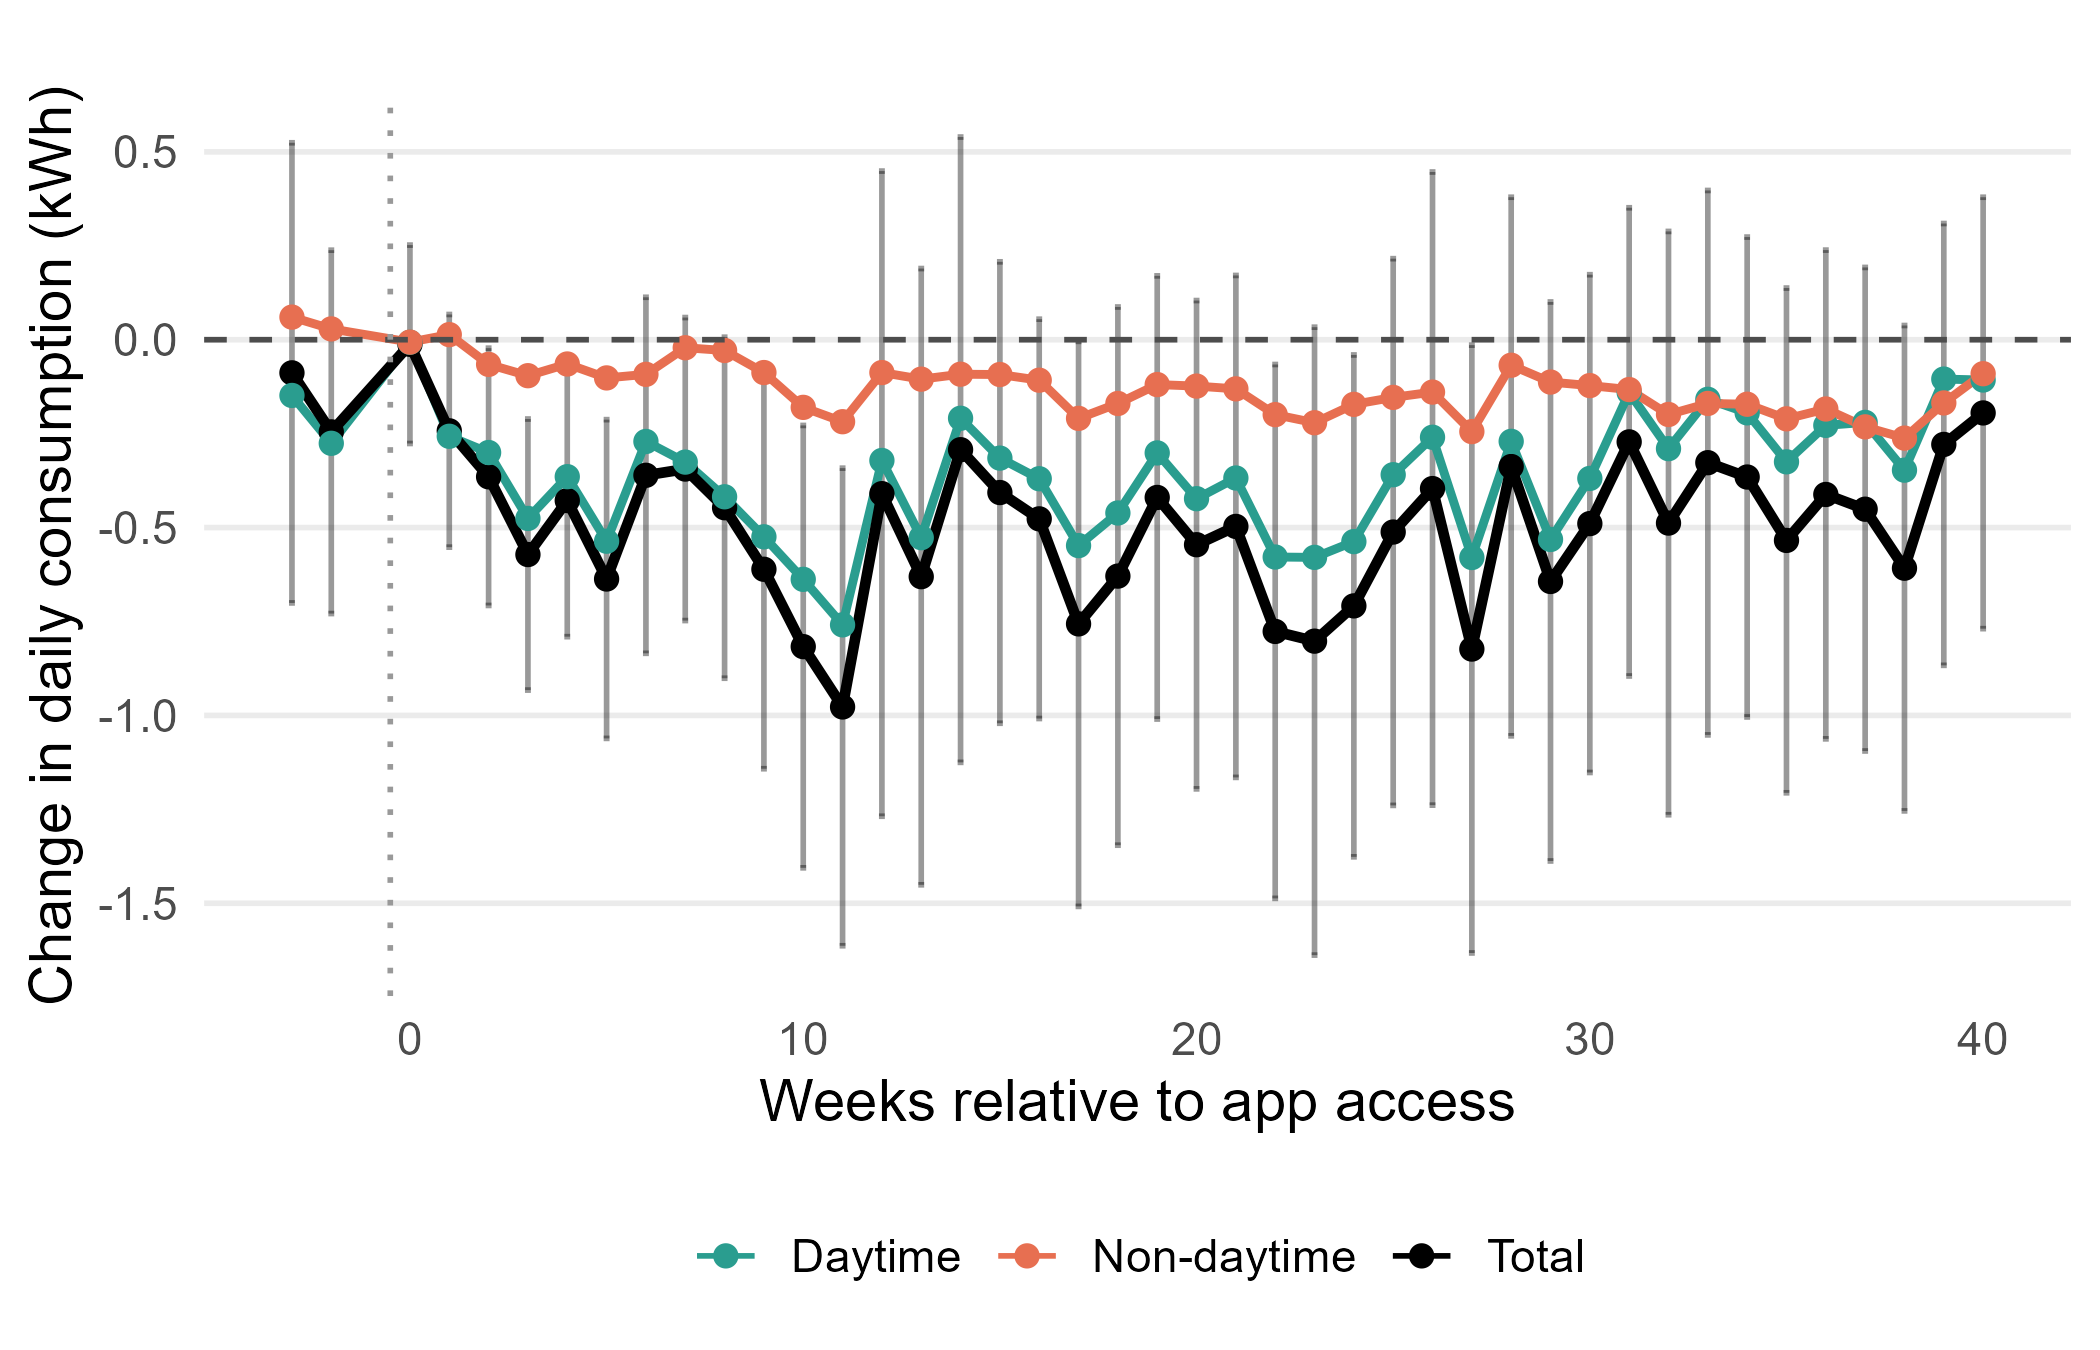
\includegraphics[width=\linewidth]{paper/figures/event_study_consumption.png}
    \caption{Dynamic treatment effects of app access on electricity consumption. The figure shows weekly event-study coefficients relative to the week prior to treatment. The black line represents total consumption, while green and orange lines denote daytime and non-daytime consumption, respectively. Vertical bars indicate 95\% confidence intervals for the total effect.}
    \label{fig:event_study}
\end{figure}

\subsection{App usage}

We next examine heterogeneity in treatment effects by  app usage. This analysis speaks to our third research question whether the time profile of treatment effects coincides with the time profile of app engagement? Because engagement is measured after treatment assignment, it is a post-treatment outcome and may reflect unobserved household characteristics such as motivation, environmental concern, or general responsiveness to feedback. The following results should therefore be interpreted as descriptive evidence on treatment dynamics rather than as causal.

We classify households into four engagement groups based on their observed app activity during the post-treatment period: high (N = 92), medium (N = 98), low (N = 104), and never (N = 155). For the purposes of the analysis, we combine never-users with the control group, thereby defining a common baseline of households without effective exposure to the app.

Table \ref{table:engagement_results} shows how treatment effects vary across engagement groups. A clear pattern emerges: reductions in electricity consumption are concentrated among households that interact more intensively with the application. The Sun--Abraham estimates indicate that highly engaged households reduce their consumption by approximately 12.5\%, while the effects for medium- and low-engagement households are smaller and not statistically distinguishable from zero. 

This pattern aligns closely with the dynamic evidence presented above. In the event-study analysis, the strongest reductions in electricity consumption occur in the period following active interaction with the app, suggesting that the effectiveness of the intervention depends not only on access to information, but also on the extent to which households attend to and process that information. Table \ref{table:engagement_results} also reports estimates from a simpler TWFE specification. These results are qualitatively similar, albeit somewhat smaller in magnitude, and support the overall pattern.

\begin{table}[H]
\centering
\caption{Treatment Effects by Engagement Level}
\label{table:engagement_results}
\begin{threeparttable}
\begin{tabular}{lccc}
\toprule
 & High & Medium & Low \\
\midrule

\textbf{Sun--Abraham ATT} \\
ATT 
& -0.1284** 
& -0.0506 
& 0.0181 \\
& (0.0392) 
& (0.0368) 
& (0.0455) \\

\addlinespace
\textbf{TWFE (OLS)} \\
Treatment effect 
& -0.0883*** 
& -0.0296 
& 0.0175 \\
& (0.0252) 
& (0.0270) 
& (0.0292) \\

\midrule
Observations 
& 269{,}989 
& 273{,}553 
& 274{,}205 \\

Household FE & Yes & Yes & Yes \\
Time FE & Day & Day & Day \\

\bottomrule
\end{tabular}

\begin{tablenotes}[flushleft]
\footnotesize
\item The dependent variable is $\log(\text{consumption} + 1)$. Columns report results for high-, medium-, and low-engagement households, respectively. Sun--Abraham estimates report aggregated average treatment effects from staggered difference-in-differences models. TWFE estimates are based on OLS regressions with an interaction between treatment assignment and the post-treatment period. All regressions include household and day fixed effects. Standard errors clustered at the household level are reported in parentheses. Significance levels: *** $p<0.01$, ** $p<0.05$, * $p<0.10$.
\end{tablenotes}

\end{threeparttable}
\end{table}

\subsection{Interpretation and economic relevance}

The results show that, on average, access to the app reduces household electricity consumption. This effect is concentrated in daytime consumption, indicating that households primarily adjust along margins over which they have greater short-term control. Treatment effects are strongest among highly engaged households, while dynamic estimates suggest gradual attenuation over time. These findings are consistent with the salience framework outlined in Section 2. According to this framework, households may consume more electricity than they would if they had access to fully salient information, if the costs of electricity use are delayed, aggregated, or difficult to attribute to specific activities. By making consumption, monetary costs and emissions more visible, the app may encourage households to make consumption choices similar to those they would make with more salient information. The concentration of effects during daytime hours is also consistent with this interpretation since adjustments should be easier to make along the margins over which households have short-term control. The gradual attenuation of effects is also consistent with the framework: if engagement only raises the salience of electricity costs while households are actively attending to the information, a decline in engagement may be associated with a return to pre-treatment behavior. While the experiment identifies the effect of offering access to the app to households registered for the study, it does not directly estimate the effects on welfare or the deadweight loss from low salience. Lower electricity consumption improves welfare if it reflects better-informed choices, but not if it reflects reductions in valued electricity services.

Taken together, the concentration of effects in daytime consumption and the co-movement of treatment effects with engagement appear more consistent with a salience channel than with pure habit formation: had households formed durable habits, reductions would be expected to persist even as engagement declines. We cannot, however, rule out a combination of channels operating simultaneously.

The estimated reduction in electricity use is modest for individual households. Using a baseline treatment effect of $0.47$\,kWh per household per day and an average electricity price of \euro{}$0.1677$ per kWh, the implied reduction in electricity expenditure amounts to approximately \euro{}$0.08$ per day, or about \euro{}$28.75$ per year per household. For the $449$ households assigned to the information condition in the analysis sample, this equates to approximately \euro{}$12{,}910$ per year. 

Because this figure aggregates the intention-to-treat effect across all households assigned to the information condition---including the 34.5\% who never used the app---it understates the savings among active users.

Using a conversion factor of $130$\,grams of CO\textsubscript{2} per kWh,\footnote{The conversion factor may differ across regions because the electricity mix varies. We use the average conversion factor for Austria in 2018.} the estimated reduction corresponds to approximately $22.3$\,kg of CO\textsubscript{2} per household per year and around $10.0$\,tonnes for treated households in the analysis sample.

These calculations describe the economic and environmental magnitude of the estimated treatment effect within the study sample. They should not be interpreted as population-level estimates. Participation required active registration and app installation, so the sample is likely to consist of more engaged and technologically inclined households than average. Consequently, the results are most informative about the effect of digital feedback among households willing to participate in such an intervention rather than about the effect of a population-wide rollout. Relative to the Upper Austrian and Austrian populations, our sample is more likely to own their dwelling (76\% vs.\ 49\% nationally), to use a heat pump for heating (31\% vs.\ 10\%), and to own a computer (98\% vs.\ 73\%; Appendix Table~\ref{tab:sample_comparison}). The findings are therefore most informative for relatively affluent and technologically engaged households.


